%\documentclass[A4,12pt]{article}
\documentclass[letterpaper,12pt]{article}
\usepackage{epsfig}
\usepackage{float}
\usepackage{amssymb,amsmath,latexsym}
\usepackage[labelformat=empty]{caption}
\usepackage{color}
%\usepackage[abs]{overpic}

\usepackage{graphicx}
\usepackage{epstopdf}

\usepackage{tikz}
\usetikzlibrary{arrows}
\usetikzlibrary{calc}
\usetikzlibrary{scopes}
\usetikzlibrary{shadows}
\usetikzlibrary{chains}
%\usetikzlibrary{shadows.blur}

\topmargin      0in 
\textheight     9.0in 
\headheight     -0.0in 
\headsep        0in
\textwidth      6.5in 
\oddsidemargin  0in 
\evensidemargin 0in
\parskip        0pt

\newcommand{\slfrac}[2]{\left.#1\middle/#2\right.}
\newcommand{\bm}    [1]{\mbox{\boldmath $#1$}}

\newtheorem{thm}           {Theorem}
\newtheorem{lemma}    [thm]{Lemma}
\newtheorem{prop}     [thm]{Proposition}
\newtheorem{property} [thm]{Property}
\newtheorem{defin}    [thm]{Definition}
\newtheorem{corollary}     {Corollary}

\begin{document}
  \noindent COM 5165 Multiple Antenna Communication \hfill 113064501 Chun-Ting Lin\\

  \begin{center}
    {\bf \large  Homework III}
  \end{center}


  %--------------------------------------------------------------
  \begin{enumerate}
    \item[{\bf 2. }]  \textbf{$\epsilon$-outage probability} \hfill \\
      The radiation pattern is obtained by projecting onto the target steering vector.
Suppose the incidence angle of the desired signal is $\phi_0$, the attenuation at angle 
$phi$ is
\begin{equation*}
    \text{P}\left(\phi\right) = \left|e_r^{H}(\Omega) \cdot e_r(\Omega_0)\right|
\end{equation*}
where
\begin{equation*}
    \Omega = \cos\left(\phi\right) \quad \text{and} \quad \Omega_0 = \cos\left(\phi_0\right)
\end{equation*}
The radiation patterns are shown below:
\begin{figure}[H]
    \centering
    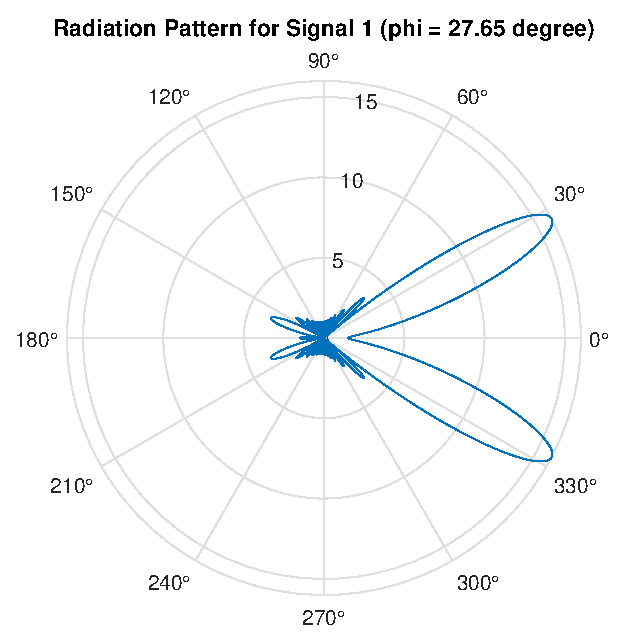
\includegraphics[scale = 0.7]{s1.eps}
\end{figure}
\begin{figure}[H]
    \centering
    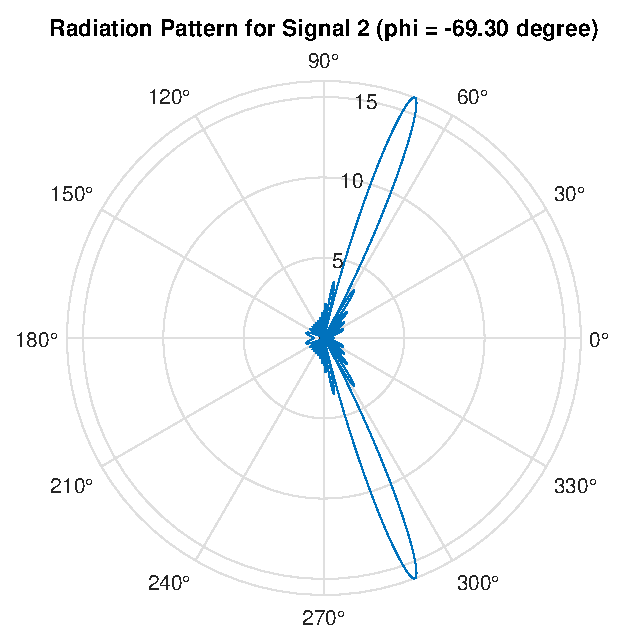
\includegraphics[scale = 0.7]{s2.eps}
\end{figure}
\begin{figure}[H]
    \centering
    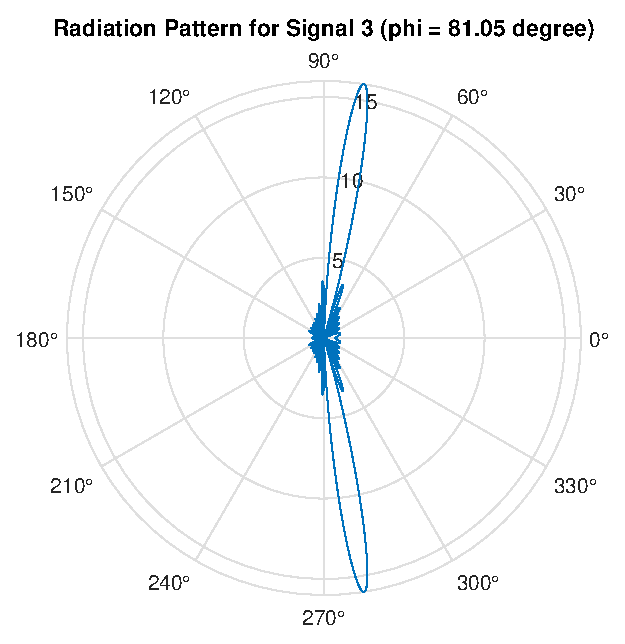
\includegraphics[scale = 0.7]{s3.eps}
\end{figure}
\begin{figure}[H]
    \centering
    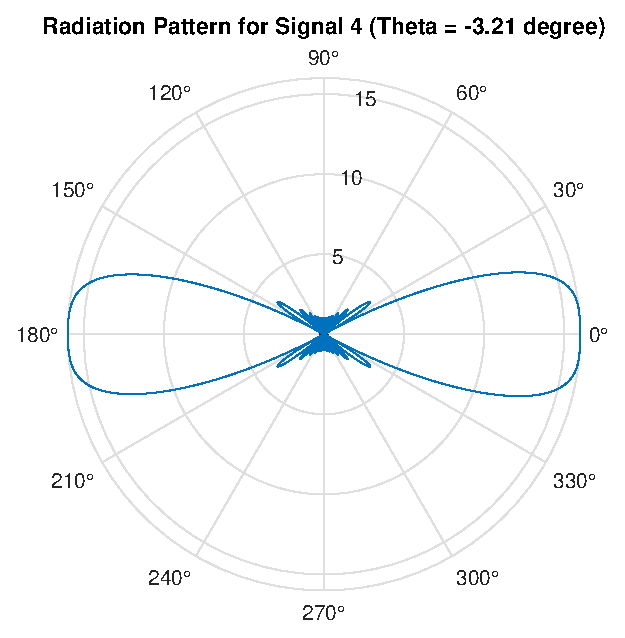
\includegraphics[scale = 0.7]{s4.eps}
\end{figure}
\begin{figure}[H]
    \centering
    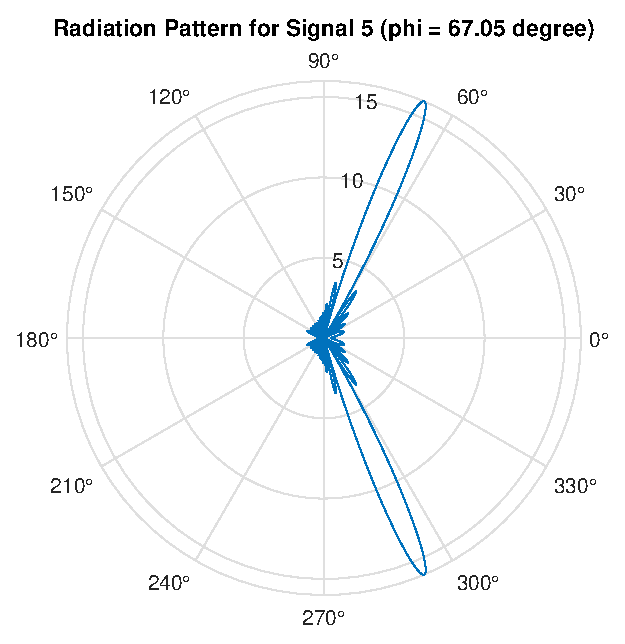
\includegraphics[scale = 0.7]{s5.eps}
\end{figure}
It can be observed that with receive beamforming, the main lobe is aligned with the incidence angle.
  \end{enumerate}
\end{document}
